
\chapter{Návrh systému a hardwarová realizace}
\label{chap:navrh-systemu}

\section{Celková architektura systému}
\label{sec:celkova-architektura}

Navržený systém byl koncipován jako bilaterální teleoperační řetězec v konfiguraci Leader--Follower. Na straně operátora byla použita haptická rukavice Remote Feelings, která představovala řídicí rozhraní Leader. Na straně vykonávací části byla použita robotická ruka InMoov, která představovala vzdálený systém Follower. Tímto uspořádáním bylo umožněno přenášet pohybový záměr uživatele směrem k robotické ruce a současně přenášet informaci o kontaktu zpět do rukavice \cite{GIUDICI2025}.

Systém byl rozdělen do dvou fyzicky oddělených subsystémů propojených bezdrátovým spojem Bluetooth Classic. Subsystém rukavice byl řízen deskou ESP32-DevKitC V4 32U. Subsystém robotické ruky byl řízen deskou Arduino UNO, ke které byl připojen modul HC-05. Komunikace byla navržena jako asynchronní full-duplex spojení s binárně kódovanými pakety. Textový formát dat nebyl použit, protože by zvyšoval objem přenášených dat a latenci komunikačního řetězce \cite{Wu2024613}.

V realizované sestavě byly použity tyto hlavní části:

\begin{itemize}
    \item \textbf{ESP32-DevKitC V4} -- řídicí jednotka rukavice Remote Feelings; byly na ní zpracovávány signály FSR, polohové signály prstů, signál sEMG, lokální asistence prstů a haptická odezva,
    \item \textbf{Arduino UNO} -- řídicí jednotka robotické ruky InMoov; byly na ní přijímány řídicí pakety, řízeny servomotory a vyhodnocovány proudy jednotlivých serv,
    \item \textbf{HC-05} -- modul Bluetooth Classic připojený k hardwarovému UARTu Arduino UNO; ESP32 vystupovalo jako Bluetooth Master,
    \item \textbf{servomotory MG996R} -- pět aktuátorů robotické ruky InMoov napájených z odděleného výkonového zdroje 5--6\,V,
    \item \textbf{senzory INA219} -- pět proudových senzorů pro odhad zatížení servomotorů a detekci kontaktu,
    \item \textbf{senzory FSR} -- pět silově citlivých rezistorů v rukavici pro vyhodnocení lokálního pohybového záměru uživatele,
    \item \textbf{potenciometry, H-můstky a DC motory z upravených serv MG90S} -- prvky použité pro snímání polohy prstů a aktivní odpor v rukavici,
    \item \textbf{senzor MyoWare 1.0} -- analogový senzor povrchové elektromyografie pro doplňkové řízení robotické ruky signálem sEMG\@.
\end{itemize}

Přenos dat byl realizován oběma směry. Z ESP32 do Arduino UNO byly odesílány cílové úhly servomotorů, hodnoty sEMG a zvolený režim řízení. Z Arduino UNO do ESP32 byly odesílány aktuální polohy serv, filtrované proudy, bitová maska kontaktu a intenzity kontaktu. Synchronizace paketů byla provedena dvojicí hlavičkových bajtů \texttt{0xAA} a \texttt{0xBB}. Struktury paketů byly sdíleny v hlavičkovém souboru \texttt{telemetry.h}, který musel být udržován identicky ve firmware obou mikrokontrolérů.

\section{Návrhové požadavky a omezení}
\label{sec:pozadavky-omezeni}

Před návrhem systému byly stanoveny požadavky vyplývající z cíle práce. Sestava neměla sloužit pouze jako jednostranné dálkové ovládání robotické ruky, ale jako obousměrný teleoperační systém umožňující řízení, měření a zpětnovazební odezvu. Základní požadavky jsou shrnuty v tabulce~\ref{tab:pozadavky-system}.

\begin{table}[htbp]
\centering
\caption{Návrhové požadavky na realizovaný systém}
\label{tab:pozadavky-system}
\begin{tabular}{|p{0.32\textwidth}|p{0.58\textwidth}|}
\hline
\textbf{Požadavek} & \textbf{Důvod a dopad na návrh} \\
\hline
Pět samostatně ovládaných prstů & Robotická ruka i rukavice obsahovaly pět prstových kanálů. V režimu MIRROR byla poloha každého prstu přenášena samostatně, zatímco režim EMG byl omezen jedním sEMG kanálem. \\
\hline
Obousměrná komunikace & Do robotické ruky bylo nutné přenášet řídicí data a zpět do rukavice proudovou telemetrii i kontaktní informaci. \\
\hline
Nízká latence & Pohyb robotické ruky a haptická odezva měly být vnímány jako spojitá reakce systému. \\
\hline
Bezpečné chování při poruše & Při resetu ESP32, výpadku Bluetooth nebo nedokončeném paketu nesměl nastat nekontrolovaný pohyb motorů ani dlouhodobé sevření robotické ruky. \\
\hline
Oddělení výkonové a řídicí části & Servomotory byly napájeny z externího zdroje. Se signálovou elektronikou byla sdílena zem, ale proudové špičky nebyly vedeny přes USB ani přes desku Arduino UNO\@. \\
\hline
Kalibrace pro aktuálního uživatele & Poloha prstů, přítlak FSR senzorů i rozsah sEMG se měnily podle nasazení rukavice a kontaktu elektrod s pokožkou. \\
\hline
Využití dostupného hardwaru & Návrh byl omezen použitými deskami, modulem HC-05, servomotory MG996R, upravenými servy MG90S a proudovými senzory INA219. \\
\hline
\end{tabular}
\end{table}

Z uvedených požadavků vyplynul kompromis mezi jednoduchostí a robustností. Na Arduino UNO byla ponechána pouze časově kritická a jednodušší část úlohy: příjem paketů, řízení serv, měření proudů a odesílání telemetrie. Na ESP32 byla umístěna výpočetně náročnější část, zejména čtení senzorů rukavice, kalibrace, aktivní asistence, sEMG zpracování a haptická reakce.

\section{Tok signálu v systému}
\label{sec:tok-signalu}

Tok signálů byl rozdělen podle provozních režimů. V režimu MIRROR byla poloha prstů snímána potenciometry v rukavici, převedena na cílové úhly a odeslána do robotické ruky. V režimu EMG byl pohybový povel odvozen ze signálu povrchové elektromyografie. V obou režimech byla na straně robotické ruky současně měřena proudová odezva servomotorů a tato informace byla využita pro odhad kontaktu.

Schématicky lze celý řetězec popsat následovně:

\begin{enumerate}
    \item v rukavici byly snímány polohy prstů, lokální zatížení FSR senzorů a sEMG signál,
    \item na ESP32 byla provedena kalibrace, filtrace a výběr režimu řízení,
    \item binární paket byl odeslán přes Bluetooth Classic do Arduino UNO,
    \item na Arduino UNO byly vypočteny řídicí pulzy serv robotické ruky,
    \item proud každého serva byl měřen senzorem INA219 a filtrován,
    \item při detekci nadproudu byl vytvořen kontaktový stav a intenzita kontaktu,
    \item telemetrický paket byl odeslán zpět do ESP32,
    \item v rukavici byla podle kontaktové informace aktivována haptická stěna.
\end{enumerate}

Do výstupního souboru nebyly vloženy externí příkazy typu \texttt{\textbackslash input}, protože by vyžadovaly doplňkové soubory a balíčky TikZ, které nejsou v hlavním souboru práce načteny. Pro vložení grafických schémat lze v další fázi použít samostatné obrázky nebo diagramy až po doplnění potřebných balíčků do preambule hlavního dokumentu.

\section{Přehled zapojení a pinout}
\label{sec:pinout}

Přehled pinů byl sestaven podle finálního firmwaru. Na straně ESP32 bylo v programu použito interní pořadí prstů malíček, prsteník, prostředník, ukazovák a palec. Na straně Arduino UNO bylo pořadí serv odlišné: palec, ukazovák, prostředník, prsteník a malíček. Převod mezi těmito konvencemi byl řešen v komunikační vrstvě.

\begin{table}[htbp]
\centering
\caption{Pinout ESP32-DevKitC V4 v rukavici Remote Feelings}
\label{tab:pinout-esp32}
\begin{tabular}{|p{0.15\textwidth}|p{0.17\textwidth}|p{0.17\textwidth}|p{0.26\textwidth}|p{0.15\textwidth}|}
\hline
\textbf{Prst} & \textbf{FSR ADC} & \textbf{Poloha ADC} & \textbf{H-můstek IN1/IN2} & \textbf{Poznámka} \\
\hline
Malíček & GPIO36 & GPIO4 & GPIO17 / GPIO16 & GPIO36 je pouze vstup. \\
\hline
Prsteník & GPIO39 & GPIO26 & GPIO22 / GPIO21 & GPIO39 je pouze vstup. \\
\hline
Prostředník & GPIO34 & GPIO27 & GPIO18 / GPIO19 & GPIO34 je pouze vstup. \\
\hline
Ukazovák & GPIO35 & GPIO14 & GPIO23 / GPIO5 & GPIO35 je pouze vstup. \\
\hline
Palec & GPIO32 & GPIO13 & GPIO12 / GPIO15 & ADC vstup ESP32. \\
\hline
\end{tabular}
\end{table}

\begin{table}[htbp]
\centering
\caption{Další signály na straně ESP32}
\label{tab:pinout-esp32-dalsi}
\begin{tabular}{|p{0.30\textwidth}|p{0.22\textwidth}|p{0.38\textwidth}|}
\hline
\textbf{Signál} & \textbf{Pin ESP32} & \textbf{Poznámka} \\
\hline
sEMG MyoWare SIG & GPIO33 (ADC1) & Byl použit vstup ADC1, protože ADC2 může být omezen při aktivním bezdrátovém spojení. \\
\hline
USB Serial monitor & USB převodník desky & Rychlost 115200 Bd; rozhraní bylo využito pro ovládací příkazy a ladění. \\
\hline
Bluetooth Classic & interní rádio ESP32 & ESP32 bylo nakonfigurováno jako Bluetooth Master a připojovalo se k MAC adrese HC-05. \\
\hline
\end{tabular}
\end{table}

\begin{table}[htbp]
\centering
\caption{Pinout Arduino UNO v robotické ruce InMoov}
\label{tab:pinout-arduino}
\begin{tabular}{|p{0.27\textwidth}|p{0.21\textwidth}|p{0.42\textwidth}|}
\hline
\textbf{Funkce} & \textbf{Pin Arduino UNO} & \textbf{Poznámka} \\
\hline
Servo palce & D8 & Řídicí pulzy serva MG996R. \\
\hline
Servo ukazováku & D9 & Řídicí pulzy serva MG996R. \\
\hline
Servo prostředníku & D2 & Řídicí pulzy serva MG996R. \\
\hline
Servo prsteníku & D3 & Řídicí pulzy serva MG996R. \\
\hline
Servo malíčku & D4 & Řídicí pulzy serva MG996R. \\
\hline
HC-05 TX $\rightarrow$ Arduino RX & D0 & Přijímaná data z modulu Bluetooth. \\
\hline
Arduino TX $\rightarrow$ HC-05 RX & D1 & Bylo použito přizpůsobení úrovní odporovým děličem 1\,k$\Omega$ / 2\,k$\Omega$. \\
\hline
I2C SDA & A4 & Společná sběrnice pro pět modulů INA219. \\
\hline
I2C SCL & A5 & Společná sběrnice pro pět modulů INA219. \\
\hline
\end{tabular}
\end{table}

\begin{table}[htbp]
\centering
\caption{Napájecí větve a společná zem systému}
\label{tab:napajeci-vetve}
\begin{tabular}{|p{0.32\textwidth}|p{0.58\textwidth}|}
\hline
\textbf{Větev} & \textbf{Zapojení a význam} \\
\hline
Logika ESP32 a senzory rukavice & ESP32 bylo napájeno přes USB nebo stabilizovaný vstup. Senzor MyoWare i analogové děliče FSR byly napájeny napětím 3,3\,V, aby nebyly překročeny vstupní limity ADC. \\
\hline
Motory a H-můstky rukavice & Výkonová část byla vedena odděleně od signálových vodičů. Řídicí vstupy H-můstků byly staženy rezistory 10\,k$\Omega$ k zemi. \\
\hline
Arduino UNO a HC-05 & Arduino UNO napájelo logickou část a modul HC-05. Modul HC-05 byl připojen na D0/D1, proto musel být při nahrávání firmware odpojen. \\
\hline
Serva InMoov & Servomotory MG996R byly napájeny z externího zdroje 5--6\,V. Kvůli proudovým špičkám byla vhodná proudová rezerva 10--15\,A. \\
\hline
Společná zem & Všechny signálové části a výkonové zdroje musely sdílet GND, aby byly definovány úrovně PWM, UART i I2C signálů. \\
\hline
\end{tabular}
\end{table}

\section{Snímací část asistivní rukavice}
\label{sec:snimaci-cast-rukavice}

Snímací část rukavice byla tvořena třemi modalitami: silově citlivými rezistory FSR, polohovými potenciometry z upravených servomechanismů a senzorem povrchové elektromyografie MyoWare 1.0. FSR senzory byly použity pro lokální asistenci prstů, potenciometry pro polohové řízení režimu MIRROR a sEMG senzor pro alternativní řízení robotické ruky.

\subsection{Silově citlivé senzory FSR}
\label{subsec:fsr}

Na každý prst rukavice byl umístěn silově citlivý rezistor. Tímto senzorem nebyla měřena svalová kontrakce přímo, ale změna mechanického tlaku nebo deformace v konstrukci rukavice. Pohybový záměr uživatele byl z hodnoty FSR pouze odvozován: při snaze prst zavřít nebo otevřít se změnilo zatížení konstrukce a tato změna byla vyhodnocena firmwarem ESP32 \cite{Trajlinek2021,GIUDICI2025}.

Senzory byly zapojeny do dělicího obvodu s referenčním rezistorem a výstupní napětí bylo přivedeno na dvanáctibitové ADC vstupy ESP32. Surové hodnoty byly během kalibrace přiřazeny ke klidovému stavu, směru zavírání a směru otevírání. Před vyhodnocením byl signál filtrován exponenciálním klouzavým průměrem
\begin{equation}
    y_k = \alpha x_k + \left(1 - \alpha\right)y_{k-1},
\end{equation}
kde $\alpha$ označuje filtrační konstantu zvolenou podle frekvence řídicí smyčky.

Výstup filtru byl porovnáván s adaptivní mrtvou zónou \texttt{DEADZONE[i]}. Její hodnota byla odvozena z klidového šumu senzoru podle vztahu
\begin{equation}
    \mathrm{DEADZONE}_i =
    \mathrm{constrain}\left(6\Delta_{\mathrm{šum}},\;15,\;150\right),
\end{equation}
kde $\Delta_{\mathrm{šum}}$ představuje rozsah špička--špička ve fázi klidové kalibrace. Touto úpravou byly potlačeny falešné aktivace způsobené elektrickým a mechanickým šumem.

\subsection{Polohové potenciometry a H-můstky}
\label{subsec:potenciometry-hmustky}

Poloha každého prstu rukavice byla snímána potenciometrem získaným z upraveného servomotoru MG90S 180$^\circ$. Běžný servomechanismus byl rozdělen na tři samostatně využitelné části: potenciometr, DC motor a řídicí H-můstek. Potenciometr byl vyveden na vstupy ADC ESP32, zatímco DC motor a H-můstek byly použity pro aktivní působení na prst rukavice.

Každý prst měl v paměti uložené krajní kalibrační hodnoty \texttt{fingerPosMin[]} a \texttt{fingerPosMax[]}. U prostředníku a ukazováku byl z mechanických důvodů směr potenciometru obrácen, takže bylo nutné v softwaru zohlednit i případ \texttt{fingerPosMin > fingerPosMax}. Řídicí signály pro H-můstky byly vedeny z ESP32 na vstupy IN\@. Na těchto vodičích byly osazeny pull-down rezistory 10\,k$\Omega$, aby při resetu ESP32 nebo při nahrávání firmware nevznikal nedefinovaný stav vedoucí k samovolnému pohybu motorů \cite{Safran2022}.

\subsection{Senzor povrchové elektromyografie MyoWare 1.0}
\label{subsec:myoware}

Pro alternativní režim řízení byl integrován analogový senzor povrchové elektromyografie MyoWare 1.0. Výstup senzoru byl přiveden na GPIO33, tedy na vstup ADC1 desky ESP32 \cite{espressif_adc}. Tato volba byla zvolena kvůli stabilnějšímu měření při současně aktivním bezdrátovém spojení. Původně uvažovaný vstup GPIO25 patří k ADC2, jehož použití může být při práci s bezdrátovou částí ESP32 problematické.

Senzor byl napájen z pinu 3V3. Napájení z 5\,V nebylo použito, protože výstup SIG by při maximální svalové kontrakci mohl dosáhnout 5\,V a překročit maximální povolené vstupní napětí ADC ESP32.

\begin{table}[htbp]
\centering
\caption{Zapojení senzoru MyoWare 1.0 k desce ESP32-DevKitC V4}
\label{tab:myoware}
\begin{tabular}{|p{0.20\textwidth}|p{0.25\textwidth}|p{0.45\textwidth}|}
\hline
\textbf{Pin MyoWare} & \textbf{Pin ESP32} & \textbf{Poznámka} \\
\hline
\texttt{+} (VCC) & \texttt{3V3} & Napájení 3,3\,V. \\
\hline
\texttt{-} (GND) & \texttt{GND} & Společná zem se systémem. \\
\hline
\texttt{SIG} & GPIO33 (ADC1) & Analogový vstup pro sEMG signál. \\
\hline
\end{tabular}
\end{table}

\section{Haptická rukavice Remote Feelings}
\label{sec:hapticka-rukavice}

Rukavice Remote Feelings byla použita jako aktivní rozhraní na straně operátora \cite{Nezval2011}. Každý prst byl vybaven DC motorem z upraveného serva MG90S a H-můstkem A3909. Motor působil na lanko připojené k článkům prstu rukavice. Pohyb v jednom směru napomáhal zavírání prstu a pohyb v opačném směru napomáhal otevírání.

Firmware ESP32 přiřazoval každému prstu stav asistence podle filtrované hodnoty FSR:

\begin{itemize}
    \item hodnota $+1$ označovala záměr zavírat prst,
    \item hodnota $-1$ označovala záměr otevírat prst,
    \item hodnota $0$ označovala klidový stav uvnitř mrtvého pásma.
\end{itemize}

Znaménko asistence bylo dále násobeno polaritou motoru uloženou v poli \texttt{MOTOR\_POLARITY[5]}. Tím byly kompenzovány mechanické rozdíly mezi jednotlivými prsty bez nutnosti přepojení vodičů.

Při detekci kontaktu robotického prstu s objektem byla v ESP32 aktivována haptická stěna. Aktuální poloha prstu v rukavici byla uložena jako hranice, za kterou mělo další zavírání vyvolat odpor. Pokud se uživatel pokoušel pokračovat v zavírání prstu, motor v rukavici působil proti tomuto pohybu. Otevření prstu nebo vypršení kontaktového okna haptickou stěnu zrušilo.

Intenzita odporu byla odvozena z hodnoty \texttt{contactIntensity} v rozsahu 0--255. Výsledná hodnota PWM byla určena vztahem
\begin{equation}
    \mathrm{PWM} =
    \mathrm{PWM}_{\min} +
    \frac{\mathrm{intenzita}}{255}
    \left(\mathrm{PWM}_{\max} - \mathrm{PWM}_{\min}\right).
\end{equation}
Pro jednotlivé prsty byly použity minimální hodnoty PWM 250, 230, 230, 250 a 250 a maximální hodnoty 650, 550, 550, 650 a 650 z rozsahu 0--1023. Haptický odpor byl tímto způsobem omezen na předem nastavený bezpečný rozsah.

\section{Robotická ruka InMoov a řídicí elektronika}
\label{sec:roboticka-ruka}

Robotická ruka InMoov byla použita jako 3D tisknutelná open-source robotická ruka s lankovým převodem pohybu prstů \cite{InMoov}. Každý prst byl ovládán jedním servomotorem MG996R umístěným v předloktí. Řídicí jednotkou byla deska Arduino UNO s mikrokontrolérem ATmega328P.

\subsection{Servomotory MG996R}
\label{subsec:mg996r}

Každý prst robotické ruky byl ovládán servomotorem MG996R s kovovými převody. Podle technických údajů dosahuje servo momentu 9,4\,kg$\cdot$cm při 4,8\,V a 11\,kg$\cdot$cm při 6\,V. Proud při zablokovaném motoru je uváděn přibližně 2,5\,A při 6\,V \cite{mg996r_towerpro}. Při současném záběru pěti serv by proto mohl okamžitý proud překročit 12\,A.

Servomotory proto nebyly napájeny z USB ani z pinu 5\,V desky Arduino UNO\@. Byl použit samostatný výkonový zdroj 5--6\,V se společnou zemí s řídicí elektronikou. Pro opakovatelný provoz byla uvažována proudová rezerva 10--15\,A. K napájecí sběrnici byl doplněn elektrolytický kondenzátor 1000\,$\mu$F / 16\,V pro potlačení krátkých proudových špiček.

Řízení serv bylo ve finální implementaci provedeno standardní knihovnou \texttt{Servo.h}. Modul HC-05 byl připojen na hardwarový UART D0/D1, takže nebyla použita knihovna \texttt{SoftwareSerial}. Tím byl odstraněn konflikt mezi softwarovou sériovou linkou a přesným časováním řídicích pulzů serv. Nevýhodou tohoto zapojení byla nutnost odpojit HC-05 při nahrávání firmware.

\subsection{Senzory proudu INA219}
\label{subsec:ina219}

Proudový odběr každého servomotoru byl měřen modulem INA219. Pět modulů bylo zapojeno paralelně na I2C sběrnici Arduino UNO, kde SDA odpovídá pinu A4 a SCL pinu A5 \cite{Lebosse2011,ti_ina219}. Senzor INA219 měří úbytek napětí na bočníku, napětí na sběrnici a umožňuje z kalibrační hodnoty vyčítat proud. V použité knihovně byla využívána funkce \texttt{getCurrent\_mA()}.

Každý modul musel mít nastavenu odlišnou I2C adresu. Použitá konfigurace je uvedena v tabulce~\ref{tab:ina219}.

\begin{table}[htbp]
\centering
\caption{I2C adresy modulů INA219 podle prstu robotické ruky}
\label{tab:ina219}
\begin{tabular}{|p{0.25\textwidth}|p{0.25\textwidth}|p{0.30\textwidth}|}
\hline
\textbf{Prst} & \textbf{I2C adresa} & \textbf{Konfigurace A0 / A1} \\
\hline
Palec & \texttt{0x40} & GND / GND \\
\hline
Ukazovák & \texttt{0x41} & VCC / GND \\
\hline
Prostředník & \texttt{0x44} & GND / VCC \\
\hline
Prsteník & \texttt{0x45} & VCC / VCC \\
\hline
Malíček & \texttt{0x48} & GND / SDA \\
\hline
\end{tabular}
\end{table}

\subsection{Bluetooth modul HC-05 a přizpůsobení úrovní}
\label{subsec:hc05}

Bezdrátové spojení bylo realizováno modulem HC-05 v roli Bluetooth Slave \cite{Sadun2016711}. Modul byl napájen z 5\,V pinu Arduino UNO a komunikoval rychlostí 9600 Bd. Po úspěšném spárování přenášel data jako transparentní sériová linka.

Protože logické úrovně vstupu HC-05 jsou 3,3\,V a výstup Arduino UNO má úroveň 5\,V, byl na lince Arduino TX $\rightarrow$ HC-05 RX použit odporový dělič napětí
\begin{equation}
    V_{\mathrm{out}} = V_{\mathrm{in}} \frac{R_2}{R_1 + R_2}
    = 5\,\mathrm{V}\frac{2\,\mathrm{k}\Omega}{1\,\mathrm{k}\Omega + 2\,\mathrm{k}\Omega}
    = 3{,}33\,\mathrm{V}.
\end{equation}
Opačný směr HC-05 TX $\rightarrow$ Arduino RX nevyžadoval dělič, protože napětí 3,3\,V bylo Arduino UNO spolehlivě rozpoznáno jako logická úroveň HIGH.

\section{Komunikační rozhraní a struktura paketů}
\label{sec:komunikacni-rozhrani}

Komunikace mezi ESP32 a Arduino UNO byla realizována přes Bluetooth Classic SPP\@. Na straně Arduino UNO byl modul HC-05 připojen k hardwarovému UARTu rychlostí 9600 Bd \cite{hc05_components101}. Na aplikační úrovni nebyly přenášeny textové příkazy, ale binární struktury opatřené dvojicí synchronizačních bajtů.

Paket odesílaný z ESP32 do Arduino UNO je popsán v tabulce~\ref{tab:packet-esp-uno}.

\begin{table}[htbp]
\centering
\caption{Paket ESP32 $\rightarrow$ Arduino UNO}
\label{tab:packet-esp-uno}
\begin{tabular}{|p{0.28\textwidth}|p{0.18\textwidth}|p{0.13\textwidth}|p{0.31\textwidth}|}
\hline
\textbf{Pole} & \textbf{Typ} & \textbf{Jednotka} & \textbf{Význam} \\
\hline
\texttt{start1}, \texttt{start2} & 2$\times$ \texttt{uint8\_t} & -- & Synchronizace paketu; hodnoty \texttt{0xAA} a \texttt{0xBB}. \\
\hline
\texttt{servoAngles[5]} & 5$\times$ \texttt{uint8\_t} & $^\circ$ & Cílové logické úhly serv v režimu MIRROR\@. \\
\hline
\texttt{emgRaw} & \texttt{uint16\_t} & ADC & Surová hodnota sEMG z ESP32. \\
\hline
\texttt{emgMin}, \texttt{emgMax}, \texttt{emgThreshold} & 3$\times$ \texttt{float} & ADC & Kalibrační hodnoty pro režim EMG\@. \\
\hline
\texttt{calibrated} & \texttt{uint8\_t} & -- & Příznak platné kalibrace. \\
\hline
\texttt{forceFeedbackEnabled} & \texttt{uint8\_t} & -- & Povolení kontaktní detekce a haptiky. \\
\hline
\texttt{controlMode} & \texttt{uint8\_t} & -- & Režim řízení NONE, MIRROR nebo EMG\@. \\
\hline
\end{tabular}
\end{table}

Celková délka paketu z ESP32 do Arduino UNO byla 24 bajtů. Při sériové lince 9600 Bd a formátu 8N1 odpovídá samotný přenos přibližně
\begin{equation}
    t_{\mathrm{ESP}\rightarrow\mathrm{UNO}} =
    \frac{24 \cdot 10}{9600}
    \approx 25\,\mathrm{ms}.
\end{equation}

Paket odesílaný z Arduino UNO do ESP32 je popsán v tabulce~\ref{tab:packet-uno-esp}.

\begin{table}[htbp]
\centering
\caption{Paket Arduino UNO $\rightarrow$ ESP32}
\label{tab:packet-uno-esp}
\begin{tabular}{|p{0.28\textwidth}|p{0.18\textwidth}|p{0.13\textwidth}|p{0.31\textwidth}|}
\hline
\textbf{Pole} & \textbf{Typ} & \textbf{Jednotka} & \textbf{Význam} \\
\hline
\texttt{start1}, \texttt{start2} & 2$\times$ \texttt{uint8\_t} & -- & Synchronizace paketu; hodnoty \texttt{0xAA} a \texttt{0xBB}. \\
\hline
\texttt{servoAngles[5]} & 5$\times$ \texttt{uint8\_t} & $^\circ$ & Aktuální logické úhly serv na Arduino UNO\@. \\
\hline
\texttt{currents\_mA[5]} & 5$\times$ \texttt{int16\_t} & mA & Filtrované proudy serv měřené senzory INA219. \\
\hline
\texttt{contactMask} & \texttt{uint8\_t} & -- & Bitová maska kontaktu jednotlivých prstů. \\
\hline
\texttt{contactIntensity[5]} & 5$\times$ \texttt{uint8\_t} & -- & Intenzita kontaktu 0--255 podle nadproudu nad baseline. \\
\hline
\end{tabular}
\end{table}

Celková délka paketu z Arduino UNO do ESP32 byla 23 bajtů, což odpovídá přibližně 24\,ms samotného přenosu na UARTu 9600 Bd. Obě strany odesílaly pakety periodicky po 35\,ms, tedy s frekvencí přibližně 28,6\,Hz. Protokol neobsahoval CRC ani checksum. Poškozený nebo neúplný paket byl zahozen a přijímač se znovu synchronizoval podle hlavičky. Doplnění kontrolního součtu bylo vyhodnoceno jako vhodné budoucí rozšíření.

\section{Zpracování proudů a kontaktní detekce}
\label{sec:kontaktova-detekce-hardware}

Kontaktní detekce nebyla založena na absolutní hodnotě proudu serva, protože proud roste i při běžném pohybu, tření a napínání lanek. Proud byl proto nejprve vzorkován každých 20\,ms, převeden na absolutní hodnotu a uložen do krátké historie pěti vzorků. Z této historie byl vypočten medián, kterým byly potlačeny osamělé proudové špičky. Medián byl následně vyhlazen exponenciálním filtrem
\begin{equation}
    I_{\mathrm{filt},k} =
    \alpha I_{\mathrm{median},k}
    + \left(1 - \alpha\right)I_{\mathrm{filt},k-1},
\end{equation}
kde v implementaci platilo $\alpha = 0{,}18$.

Detekce kontaktu byla provedena z nadproudu vzhledem k adaptivní základní hladině
\begin{equation}
    I_{\mathrm{extra}} =
    \max\left(0, I_{\mathrm{filt}} - I_{\mathrm{baseline}}\right).
\end{equation}
Základní hladina byla přizpůsobována asymetricky. Při poklesu proudu byla upravována rychleji ($\alpha = 0{,}12$), při růstu pomaleji ($\alpha = 0{,}025$). Tím bylo zabráněno tomu, aby byl skutečný kontakt okamžitě pohlcen adaptací jako nová normální hodnota.

Kontakt byl potvrzen pouze tehdy, pokud byl prst v posledních 350\,ms řízen směrem k zavření a nadproud překročil 450\,mA po třech po sobě jdoucích vzorcích. Při vzorkování 20\,ms to odpovídalo minimální potvrzovací době přibližně 60\,ms. Kontakt byl uvolněn při povelu k otevření nebo po poklesu nadproudu pod 170\,mA po deseti vzorcích, tedy přibližně po 200\,ms.

Intenzita kontaktu byla počítána lineárním mapováním nadproudu do rozsahu 0--255. Spodní hranice odpovídala 170\,mA a horní hranice 1400\,mA nad adaptivní baseline. Výsledná intenzita byla dále filtrována s konstantou $\alpha = 0{,}35$ a odeslána do ESP32.

\section{Kalibrace systému}
\label{sec:kalibrace-systemu-hardware}

Kalibrace byla nutná kvůli mechanické variabilitě rukavice, odlišnému nasazení na ruku uživatele a nestabilitě analogových signálů. Kalibrační hodnoty byly ukládány do RAM, proto byly platné pouze pro aktuální běh programu. Po resetu nebo novém nahrání firmware bylo nutné kalibraci zopakovat.

\begin{table}[htbp]
\centering
\caption{Kalibrační kroky systému}
\label{tab:kalibrace-systemu}
\begin{tabular}{|p{0.28\textwidth}|p{0.62\textwidth}|}
\hline
\textbf{Kalibrace} & \textbf{Postup a význam} \\
\hline
Poloha prstů rukavice & Příkazem \texttt{c} byla změřena otevřená a sevřená poloha každého prstu. Tyto hodnoty byly použity pro převod ADC hodnot na logický úhel 0--180$^\circ$. \\
\hline
FSR senzory & Byl změřen klidový stav, rozsah při pohybu a šum. Z těchto hodnot byla odvozena mrtvá zóna. \\
\hline
Klidová síla rukavice & Příkazem \texttt{z} byly aktuální hodnoty FSR uloženy jako nový klidový stav. \\
\hline
sEMG signál & Během kalibrace byly změřeny hodnoty v klidu a při svalové aktivaci. Tyto hodnoty byly použity pro normalizaci EMG režimu. \\
\hline
Proudová baseline INA219 & Baseline nebyla nastavována jednorázově, ale adaptivně během provozu. \\
\hline
Proudové prahy kontaktu & Pro sepnutí kontaktu byl použit práh 450\,mA nad baseline a pro uvolnění 170\,mA nad baseline. \\
\hline
\end{tabular}
\end{table}

Opakovatelnost kalibrace byla ovlivněna zejména nasazením rukavice, tlakem FSR senzorů, vedením lanek a kvalitou kontaktu sEMG elektrod s pokožkou. Kalibrace proto byla zařazena jako běžná součást spuštění systému.

\section{Bezpečnostní opatření}
\label{sec:bezpecnostni-opatreni}

Bezpečnost systému byla řešena kombinací hardwarových a softwarových opatření. Na straně rukavice byly vstupy H-můstků staženy pull-down rezistory 10\,k$\Omega$ k zemi, aby při resetu ESP32 nebo při nahrávání firmware nevznikaly nedefinované stavy. Firmware ESP32 při ztrátě Bluetooth zastavil lokální motory rukavice a opakovaně se pokoušel obnovit spojení.

Na straně robotické ruky byl rozsah řídicích pulzů serv omezen hodnotami 350--2700\,$\mu$s. Každý prst měl vlastní kalibrované hodnoty otevřené a zavřené polohy. Při výpadku paketů z ESP32 delším než 500\,ms Arduino UNO zrušilo aktivní režim, vyčistilo stav kontaktu a vrátilo ruku do otevřené polohy.

Haptická odezva nebyla realizována jako tvrdé uzamčení prstu, ale jako omezený motorický odpor. PWM haptické odezvy bylo shora omezeno. Haptická stěna byla držena nejvýše 800\,ms od posledního kontaktového paketu a mohla být uvolněna otevřením prstu. Tím bylo sníženo riziko bolestivého tahu v rukavici i riziko trvalého zablokování prstu.

\section{Základní provozní a měřené hodnoty}
\label{sec:provozni-hodnoty}

Základní provozní hodnoty byly převzaty z firmwaru a z experimentálního testování. Proudové hodnoty serv v klidu, při volném pohybu a při kontaktu nebyly uváděny jako samostatná naměřená tabulka, protože nebyl k dispozici dostatečně opakovaný a validovaný soubor měření. Pro kontaktní detekci jsou proto uvedeny implementované prahy nadproudu.

\begin{table}[htbp]
\centering
\caption{Základní provozní a experimentálně zjištěné hodnoty}
\label{tab:provozni-hodnoty}
\begin{tabular}{|p{0.42\textwidth}|p{0.18\textwidth}|p{0.30\textwidth}|}
\hline
\textbf{Veličina} & \textbf{Hodnota} & \textbf{Poznámka} \\
\hline
USB Serial ESP32 & 115200 Bd & Ovládací příkazy a ladění ESP32. \\
\hline
UART Arduino UNO / HC-05 & 9600 Bd & Binární protokol mezi deskami. \\
\hline
Perioda paketů ESP32 $\rightarrow$ UNO & 35\,ms & Přibližně 28,6\,Hz. \\
\hline
Perioda paketů UNO $\rightarrow$ ESP32 & 35\,ms & Přibližně 28,6\,Hz. \\
\hline
Teoretický přenos paketu ESP32 $\rightarrow$ UNO & 25\,ms & 24 bajtů, 8N1, 9600 Bd. \\
\hline
Teoretický přenos paketu UNO $\rightarrow$ ESP32 & 24\,ms & 23 bajtů, 8N1, 9600 Bd. \\
\hline
Lokální řízení motorů rukavice & 20\,ms & Přibližně 50\,Hz. \\
\hline
Vzorkování proudů INA219 & 20\,ms & Přibližně 50\,Hz. \\
\hline
ADC ESP32 & 12 bitů & Rozsah 0--4095. \\
\hline
PWM rukavice & 5\,kHz, 10 bitů & Rozsah 0--1023. \\
\hline
Potvrzení kontaktu & 3 vzorky & Přibližně 60\,ms nad prahem. \\
\hline
Uvolnění kontaktu & 10 vzorků & Přibližně 200\,ms pod uvolňovacím prahem. \\
\hline
Práh sepnutí kontaktu & 450\,mA nad baseline & Proudový nadbytek po filtraci. \\
\hline
Práh uvolnění kontaktu & 170\,mA nad baseline & Hystereze kontaktu. \\
\hline
Držení haptické stěny & 800\,ms & Bez nového kontaktového paketu haptická stěna zanikla. \\
\hline
Průměrná reakce MIRROR při zavření & 134{,}8\,ms & Měřeno v testu otevřít--zavřít--otevřít. \\
\hline
Průměrná reakce MIRROR při otevření & 126{,}4\,ms & Měřeno v testu otevřít--zavřít--otevřít. \\
\hline
Průměrná reakce EMG při zavření & 546{,}4\,ms & Ovlivněno filtrací a nestabilitou sEMG\@. \\
\hline
Průměrná reakce EMG při otevření & 553{,}2\,ms & Ovlivněno filtrací a nestabilitou sEMG\@. \\
\hline
\end{tabular}
\end{table}

\section{Dílčí shrnutí návrhu systému}
\label{sec:shrnuti-navrhu}

Navržený systém splnil základní požadavky na obousměrnou teleoperaci mezi rukavicí a robotickou rukou. Rukavicí Remote Feelings byla snímána poloha prstů, vyhodnocována lokální snaha uživatele pomocí FSR senzorů a přijímána haptická informace z robotické ruky. Robotickou rukou InMoov byly přijímány řídicí pakety, ovládáno pět servomotorů a měřen jejich proudový odběr senzory INA219.

Hardwarová realizace současně ukázala hlavní omezení řešení. Komunikace přes HC-05 byla jednoduchá a funkční, ale rychlost 9600 Bd omezovala minimální dobu přenosu paketu. Proudová detekce kontaktu byla citlivá na tření a napnutí lanek, proto musela být doplněna filtrací, adaptivní baseline a hysterezí. Režim EMG byl omezen kvalitou jednoho analogového kanálu a jeho citlivostí na pohybové artefakty. Tyto skutečnosti byly dále rozpracovány v navazující softwarové kapitole.

\chapter{Softwarové řešení a zpracování signálů}
\label{chap:software}

\section{Celkové uspořádání softwaru}
\label{sec:celkove-usporadani-softwaru}

Software systému byl rozdělen do dvou samostatných projektů vyvíjených v prostředí PlatformIO s použitím Arduino frameworku. Projekt \textit{Remote\_Feelings\_sEMG} byl určen pro ESP32 v rukavici a projekt \textit{InMoov\_BLE\_control} byl určen pro Arduino UNO v robotické ruce. Společnou částí obou projektů byl soubor \texttt{telemetry.h}, ve kterém byly definovány struktury binárních paketů.

V implementovaném systému byly použity tři hlavní způsoby převodu vstupních signálů na pohyb nebo haptickou odezvu. Prvním bylo zrcadlení polohy prstů v režimu MIRROR\@. Druhým bylo řízení podle signálu sEMG\@. Třetím byla kontaktní detekce z proudových senzorů INA219, z níž byla odvozena haptická odezva v rukavici. Ve všech případech byla nutná kalibrace, normalizace, filtrace a hysterezní omezení, protože analogové signály byly zatíženy šumem a mechanická soustava obsahovala vůle, tření a pružné prvky.

\section{Zpracování sEMG signálu a kalibrace}
\label{sec:semg-zpracovani}

Zpracování sEMG signálu bylo založeno na kalibraci, filtraci a výpočtu aktivační proměnné s hysterezí. Tento postup odpovídá obecným principům zpracování elektromyografických signálů, u nichž je nutné potlačovat šum, artefakty a uživatelskou variabilitu \cite{DeLuca2010,Reaz2006,Chowdhury2013917}.

\subsection{Kalibrační protokol}
\label{subsec:kalibracni-protokol}

Kalibrace byla spouštěna příkazem \texttt{c} ze Serial Monitoru ESP32. Byla rozdělena do dvou fází. V první fázi byla ruka držena otevřená přibližně 3\,s. Během této doby byly průměrovány klidové hodnoty FSR senzorů, polohové hodnoty prstů a minimální hodnota sEMG\@. Současně byl měřen šum FSR senzorů, z něhož byla odvozena mrtvá zóna \texttt{DEADZONE[i]}.

Ve druhé fázi byla po dobu přibližně 5\,s opakovaně svírána ruka v pěst. Zaznamenány byly maximální hodnoty FSR, krajní polohy prstů a maximální hodnota sEMG\@. Z naměřených hodnot byl odvozen aktivační práh
\begin{equation}
    \mathrm{emgThreshold} =
    \mathrm{emgMin} + 0{,}1\left(\mathrm{emgMax} - \mathrm{emgMin}\right).
\end{equation}
Hodnota 10\,\% rozsahu od minima byla použita jako kompromis mezi rychlou odezvou a potlačením falešných aktivací v klidu.

Po kalibraci byl volitelně proveden ověřovací pohyb prstů. Každý prst přejel do otevřené a poté do zavřené polohy. Tím byla ověřena polarita motorů a mechanické meze. V blízkosti krajních poloh bylo použito kvadratické zpomalení, protože lineární brzdění způsobovalo příliš agresivní dojezd.

\subsection{Filtrace a normalizace sEMG}
\label{subsec:filtrace-semgg}

Surový sEMG signál byl zatížen náhodnými špičkami a pohybovými artefakty. Pro potlačení vysokofrekvenčních složek byl použit exponenciální klouzavý průměr
\begin{equation}
    y_k = \alpha x_k + \left(1 - \alpha\right)y_{k-1}.
\end{equation}
Na ESP32 byla použita filtrační konstanta $\alpha = 0{,}08$. Nižší hodnota byla zvolena vzhledem k vysoké frekvenci běhu smyčky mikrokontroléru a potřebě výraznějšího vyhlazení.

Při silné kontrakci mohlo dojít k přesycení filtru. Surový signál proto byl před filtrem omezen vztahem
\begin{equation}
    x_k^{\mathrm{sat}} = \min\left(x_k,\;1{,}2\,\mathrm{emgMax}\right).
\end{equation}
Tím bylo zabráněno tomu, aby filtr akumuloval extrémní hodnotu a po uvolnění svalu se vracel do klidové úrovně příliš pomalu.

Normalizovaná aktivační proměnná byla definována jako
\begin{equation}
    a = \mathrm{constrain}\!\left(
        \frac{\mathrm{EMG}_{\mathrm{raw}} - \mathrm{EMG}_{\min}}
             {\left|\mathrm{EMG}_{\max} - \mathrm{EMG}_{\min}\right|},
        0,\;1
    \right).
\end{equation}
Absolutní hodnota ve jmenovateli byla použita proto, aby systém zůstal funkční i při invertovaném průběhu sEMG signálu. Pokud byl kalibrační rozsah příliš malý, aktivace nebyla vyhodnocována, aby řízení nevznikalo pouze ze šumu.

\subsection{Hystereze a mrtvé pásmo}
\label{subsec:hystereze-semgg}

Servo reagovalo až po překročení aktivačního prahu \texttt{EMG\_ACTIVATION\_THRESHOLD}. Uvolnění bylo provedeno až po poklesu pod nižší práh \texttt{EMG\_RELEASE\_THRESHOLD}. Touto hysterezí bylo omezeno kmitání serv kolem jedné rozhodovací úrovně.

Dále bylo zavedeno mrtvé pásmo, v němž nebyla do serv zapisována nová hodnota. Stavová proměnná \texttt{isAtRest} zajistila, že přechod do klidové polohy byl proveden jednorázově a následně byl zápis do serv zastaven. Tím byl snížen proudový odběr i nežádoucí vrčení serv v klidu.

\section{Algoritmus detekce pohybového záměru v rukavici}
\label{sec:algoritmus-zameru}

Pohybový záměr uživatele byl v rukavici vyhodnocován z filtrovaných hodnot FSR senzorů. Pro každý prst byla porovnávána aktuální hodnota s kalibrovanou klidovou hodnotou a adaptivní mrtvou zónou. Pokud filtrovaná hodnota překročila \texttt{restForce[i] + DEADZONE[i]}, byl vyhodnocen záměr zavírat prst. Pokud hodnota klesla pod \texttt{restForce[i] - DEADZONE[i]}, byl vyhodnocen záměr otevírat prst. V opačném případě byl motor daného prstu zastaven.

\subsection{Releová regulace motorů rukavice}
\label{subsec:releova-regulace}

Pro řízení motorů rukavice byla použita releová regulace. Při nenulovém stavu asistence byla motoru přiřazena pevná hodnota PWM \texttt{BANGBANG\_PWM} s odpovídajícím znaménkem. Tento způsob byl zvolen kvůli odolnosti vůči šumu FSR senzorů. Nebylo nutné přesně mapovat velikost mechanického zatížení na výkon motoru; postačovalo rozhodnutí, zda je záměr pohybu přítomen.

Byly sice implementovány i proporcionální, PD a impedanční strategie, označené jako \texttt{modeProp}, \texttt{modePD} a \texttt{modeImpedance}, jejich provozní odladění však bylo výrazně komplikováno nelinearitami lanek, třením a rozdílnou mechanikou prstů. V realizované verzi proto byla použita robustnější releová varianta \cite{GIUDICI2025}.

Řídicí smyčka motorů rukavice byla spouštěna časově po 20\,ms. Mezi jednotlivými kroky byla obsluhována komunikace Bluetooth, aby nedocházelo k zahlcení nebo blokování bezdrátového zásobníku ESP32.

\subsection{Pozicová omezení a polarita motorů}
\label{subsec:pozicova-omezeni}

Každý prst měl z kalibrace uloženou otevřenou a zavřenou polohu. Funkcí \texttt{isMotorAtPositionLimit()} bylo detekováno dosažení krajní polohy, při němž byl motor zastaven bez použití samostatných koncových spínačů. U prstů s opačným směrem potenciometru bylo výpočetně ošetřeno obrácené pořadí krajních hodnot. Softwarová polarita motorů byla uložena v konfiguračních polích, takže mechanické rozdíly mohly být kompenzovány bez změny zapojení.

\section{Implementace bezdrátového komunikačního protokolu}
\label{sec:implementace-bt-protokolu}

Binární protokol byl definován v souboru \texttt{telemetry.h}. Struktury byly označeny direktivou \texttt{\_\_attribute\_\_((packed))}, aby bylo zabráněno automatickému doplňování výplňových bajtů překladačem. Tím byla zajištěna shoda velikosti struktury mezi architekturou AVR použitou v Arduino UNO a architekturou Xtensa použitou v ESP32.

Synchronizační bajty \texttt{0xAA} a \texttt{0xBB} umožňovaly detekci začátku paketu i po ztrátě bajtů. Přijímač vyhledával hlavičku a po jejím nalezení přečetl pevný počet bajtů odpovídající danému typu paketu. Protože nebyl použit kontrolní součet, nemohla být odhalena každá chyba uvnitř paketu. Pro budoucí verzi proto bylo doporučeno doplnit CRC nebo alespoň jednoduchý XOR checksum.

ESP32 vystupovalo jako Bluetooth Master a inicializovalo spojení k modulu HC-05 podle MAC adresy uložené ve firmware. MAC adresa byla zjištěna pomocí aplikace Serial Bluetooth Terminal v režimu Bluetooth Classic. Úspěšné spárování bylo signalizováno změnou blikání LED na modulu HC-05.

Během kalibrace vznikal problém s blokujícími smyčkami, které mohly zastavit obsluhu Bluetooth stacku a vyvolat reset ESP32 přes Task Watchdog Timer. Proto byly dlouhé čekací úseky nahrazeny funkcemi pro průběžnou obsluhu pozadí. Funkce \texttt{serviceBackgroundTasks()} resetovala watchdog, zpracovávala příchozí data a průběžně odesílala stav. Funkce \texttt{delayWithBackgroundTasks()} nahrazovala blokující \texttt{delay()}.

Pro potlačení zahlcení terminálu a Bluetooth zásobníku bylo do \texttt{platformio.ini} přidáno:

\begin{lstlisting}
build_flags = -DCORE_DEBUG_LEVEL=0
\end{lstlisting}

Tím byly vypnuty interní debug výpisy Bluetooth knihovny. Bez tohoto nastavení se při přetečení přijímacího bufferu objevovala hlášení typu \texttt{RX Full!}, která dále zhoršovala stabilitu komunikace.

\section{Převod dat mezi režimy řízení}
\label{sec:prevod-dat-rezimy}

V režimu MIRROR byla poloha každého prstu převáděna z ADC hodnoty na logický úhel 0--180$^\circ$. Pro převod byl použit vztah
\begin{equation}
    \theta = \mathrm{constrain}\!\left(
        \frac{x - x_{\min}}{x_{\max} - x_{\min}} \cdot 180,
        0,\;180
    \right),
\end{equation}
kde $x$ označuje aktuální ADC hodnotu a $x_{\min}$, $x_{\max}$ kalibrované krajní hodnoty. Tím byl odlišný mechanický rozsah jednotlivých prstů převeden na jednotný formát pro robotickou ruku.

V režimu EMG nebyly jednotlivé prsty řízeny nezávisle. Arduino UNO z přijaté sEMG hodnoty vypočítalo aktivační proměnnou a tuto hodnotu mapovalo na společné sevření všech prstů robotické ruky. Jeden sEMG kanál proto neumožňoval jemné a oddělené ovládání jednotlivých prstů. Toto omezení bylo zásadní při experimentálním porovnání s režimem MIRROR\@.

V lokálním režimu asistence byly motory rukavice řízeny podle FSR senzorů a tento režim mohl běžet současně s režimem MIRROR nebo EMG\@. Režim asistence nebyl přímým režimem řízení robotické ruky, ale lokálním podpůrným mechanismem v rukavici.

\section{Firmware řídicí jednotky robotické ruky}
\label{sec:firmware-roboticke-ruky}

Firmware \textit{InMoov\_BLE\_control} vykonával sekvenční smyčku s periodou přibližně 20\,ms. Ve smyčce byl střídán příjem paketů z HC-05, aktualizace servomotorů a vzorkování proudů INA219.

Arduino UNO na hardwarovém sériovém rozhraní vyhledávalo synchronizační sekvenci \texttt{0xAA}, \texttt{0xBB}. Po přijetí validního paketu byl obnoven časovač příjmu. Pokud nebyl přijat žádný platný paket po dobu delší než nastavený timeout, byl systém převeden do bezpečného režimu a ruka byla otevřena.

V režimu MIRROR byly cílové úhly převedeny na šířku řídicího pulzu serv. Výsledná hodnota byla omezena bezpečnostními mezemi \texttt{SERVO\_SAFE\_MIN\_US} a \texttt{SERVO\_SAFE\_MAX\_US}, aby nedocházelo k mechanickému přetočení \cite{Krycner2024}. Každý prst měl vlastní kalibrační hodnoty otevřené a zavřené polohy, protože mechanické uložení serv a vedení lanek nebyly u všech prstů totožné.

\section{Algoritmus silové zpětné vazby}
\label{sec:algoritmus-force-feedback}

Silová zpětná vazba byla odvozena z proudové detekce kontaktu. Po přijetí telemetrického paketu s nenulovou hodnotou \texttt{contactMask} byla pro příslušné prsty na ESP32 aktivována haptická stěna \cite{Begalinova2020,Fang2022}. Při prvním kontaktu byla uložena aktuální poloha prstu jako \texttt{hapticWallPos[i]}. Pokud se uživatel snažil prst dále zavírat, motor rukavice působil proti tomuto pohybu.

Výkon haptického odporu byl mapován z hodnoty intenzity kontaktu:
\begin{equation}
    \mathrm{PWM}_{\mathrm{haptic}} =
    \mathrm{map}\left(
        \mathrm{contactIntensity}[i],
        0,\;255,
        \mathrm{PWM}_{\min},\;\mathrm{PWM}_{\max}
    \right).
\end{equation}
Tím byl uživateli poskytnut hrubý vjem odporu proti dalšímu sevření. Systém nebyl určen k reprodukci jemné textury ani vysokofrekvenčních vibrací; pro takovou úlohu by byla nutná specializovaná vibrotaktilní aktuace s vyšší šířkou pásma \cite{Fang2022}.

Kontaktní detekci byla ve firmware přiřazena vyšší priorita než lokální asistenci. Pokud byl detekován kontakt na prstu, byla hodnota \texttt{driveSpeed[i]} přepsána haptickým odporem a běžná asistence byla dočasně potlačena. Haptická stěna zanikla po 800\,ms bez nového kontaktového paketu, aby při výpadku Bluetooth nevzniklo trvalé zablokování prstu.

Kompletní datový tok od kontaktu k haptické odezvě byl následující:

\begin{enumerate}
    \item servomotor robotické ruky narazil na objekt a jeho proud vzrostl,
    \item proud byl změřen senzorem INA219 a zpracován mediánem, EMA filtrem a adaptivní baseline,
    \item stavový automat vyhodnotil kontakt a vypočítal intenzitu 0--255,
    \item Arduino UNO odeslalo paket \texttt{UnoToEspPacket},
    \item ESP32 uložilo aktuální polohu prstu jako haptickou stěnu,
    \item při dalším zavírání prstu byl motor v rukavici aktivován proti pohybu uživatele,
    \item operátor vnímal odpor jako silovou zpětnou vazbu.
\end{enumerate}

\section{Dílčí shrnutí softwarové části}
\label{sec:shrnuti-software}

Softwarové řešení bylo navrženo jako rozdělený systém se silně oddělenými úlohami. ESP32 zajišťovalo zpracování senzorů rukavice, režim asistence, sEMG kalibraci a haptickou odezvu. Arduino UNO zajišťovalo řízení serv robotické ruky, měření proudů a kontaktní detekci. Komunikace byla provedena binárním protokolem s pevnou délkou paketů.

Největší omezení softwarové části vyplývalo z absence kontrolního součtu, omezené rychlosti UARTu 9600 Bd a citlivosti sEMG signálu na rušení. Naopak režim MIRROR byl díky přímému polohovému řízení jednodušší, stabilnější a lépe interpretovatelný. Tato rozdílná spolehlivost obou režimů byla ověřena experimentálně v následující kapitole.

\chapter{Experimentální testování a výsledky}
\label{chap:experimentalni-testovani}

\section{Cíl experimentálního testování}
\label{sec:cil-testovani}

Cílem experimentálního testování bylo ověřit funkčnost realizované sestavy robotické ruky a haptické rukavice a současně porovnat praktickou použitelnost dvou režimů řízení robotické ruky. Prvním režimem byl režim MIRROR, při kterém robotická ruka kopírovala polohu prstů snímanou rukavicí. Druhým režimem byl režim EMG, při kterém byl pohyb robotické ruky odvozován ze signálu povrchové elektromyografie.

Testování bylo provedeno dne 23.~6.~2026 ve 22:22. Testující osobou byl Bc.~Filip Vencl. Testována byla aktuální verze firmwaru pro ESP32 v rukavici Remote Feelings a pro Arduino UNO v robotické ruce InMoov Hand. Senzor sEMG byl v době testování funkční, avšak vykazoval nestabilní signál. Kontaktní detekce a silová zpětná vazba byly součástí systému, jejich samostatná validace však nebyla hlavním předmětem porovnání režimů MIRROR a EMG\@.

Experimentální část byla zaměřena především na stabilitu, rychlost, opakovatelnost, jemnou ovladatelnost a praktickou využitelnost obou režimů při manipulaci s předměty.

\section{Popis testované sestavy a režimů řízení}
\label{sec:popis-testovane-sestavy}

Testovaná sestava zahrnovala jednotku ESP32 umístěnou v rukavici Remote Feelings, Arduino UNO v robotické ruce InMoov Hand, modul HC-05 a servopohony robotické ruky. Komunikace mezi ESP32 a Arduino UNO byla během testování funkční a stabilní. Napájení serv robotické ruky zůstávalo stabilní i při vyšším proudovém odběru.

Hlavní omezení testu se projevovalo v části sEMG měření. Zapojení sEMG bylo omezeno dlouhými a nestíněnými vodiči a vlivem pohybových artefaktů. V blízkosti testovací sestavy se nacházely napájecí kabely a počítač, takže nebylo možné plně eliminovat rušení. Tyto skutečnosti byly zohledněny při interpretaci výsledků režimu EMG\@.

\begin{table}[htbp]
\centering
\caption{Použité zkratky a ovládací příkazy}
\label{tab:pouzite-zkratky-prikazy}
\begin{tabular}{|p{0.25\textwidth}|p{0.65\textwidth}|}
\hline
\textbf{Označení} & \textbf{Význam} \\
\hline
MIRROR & Řízení robotické ruky podle polohy prstů v rukavici; příkaz \texttt{q}. \\
\hline
EMG & Řízení robotické ruky podle sEMG signálu; příkaz \texttt{w}. \\
\hline
Aktivní podpora rukavice & Lokální motorová podpora na ESP32; příkaz \texttt{1}. \\
\hline
FF & Kontaktní detekce a silová zpětná vazba; příkaz \texttt{f}. \\
\hline
\end{tabular}
\end{table}

\section{Metodika testování}
\label{sec:metodika-testovani}

Testování bylo rozděleno do deseti dílčích měření označených M0 až M9. Jednotlivá měření byla navržena tak, aby bylo možné posoudit základní provozuschopnost sestavy, stabilitu systému v klidu, dynamickou odezvu robotické ruky, schopnost řízení mezilehlé polohy, praktickou manipulaci s předměty a vliv rušení na EMG řízení.

\begin{table}[htbp]
\centering
\caption{Přehled provedených měření}
\label{tab:prehled-mereni}
\begin{tabular}{|p{0.15\textwidth}|p{0.75\textwidth}|}
\hline
\textbf{Označení} & \textbf{Účel měření} \\
\hline
M0 & Úvodní kontrola sestavy. \\
\hline
M1 & Stabilita v klidu v režimu MIRROR\@. \\
\hline
M2 & Stabilita v klidu v režimu EMG\@. \\
\hline
M3 & Dynamický test otevřít--zavřít--otevřít v režimu MIRROR\@. \\
\hline
M4 & Dynamický test otevřít--zavřít--otevřít v režimu EMG\@. \\
\hline
M5 & Pokus o poloviční sevření v režimu MIRROR\@. \\
\hline
M6 & Pokus o poloviční sevření v režimu EMG\@. \\
\hline
M7 & Uchopení předmětu v režimu MIRROR\@. \\
\hline
M8 & Uchopení předmětu v režimu EMG\@. \\
\hline
M9 & Pozorování rušení EMG\@. \\
\hline
\end{tabular}
\end{table}

U testů stability v klidu byla sledována poloha robotické ruky po dobu 30~s. U dynamických testů otevření a zavření bylo provedeno pět opakování. U testů polovičního sevření byla hodnocena schopnost dosáhnout přibližně 50~\% sevření a udržet tuto polohu po dobu 5~s. Při praktickém testu uchopení byly použity tři předměty: houbička na nádobí, plastový meč a fixa.

\section{Úvodní kontrola sestavy}
\label{sec:uvodni-kontrola}

Před zahájením vlastního porovnání režimů byla provedena úvodní kontrola sestavy. Během této kontroly bylo zjištěno, že sEMG senzor byl funkční, ale jeho signál byl nestabilní. ESP32, Arduino UNO i spojení HC-05 byly funkční. Napájení serv robotické ruky bylo stabilní i při vyšším odběru. Byla provedena kalibrace příkazem \texttt{c} a následně také nastavení klidové síly příkazem \texttt{z}.

Sestava byla v době testu provozuschopná. Hlavním omezením byl nestabilní sEMG signál, pravděpodobně ovlivněný délkou a nestíněním kabeláže, blízkostí napájecích kabelů a počítače a pohybovými artefakty.

\section{Stabilita systému v klidovém stavu}
\label{sec:stabilita-klid}

Stabilita v klidovém stavu byla ověřována samostatně pro režim MIRROR a režim EMG\@. Cílem bylo zjistit, zda robotická ruka zůstává v klidu bez nežádoucích pohybů a zda se případné nestability projevují spíše v řídicím režimu, komunikaci, mechanice nebo vstupním signálu.

\subsection{Stabilita v klidu v režimu MIRROR}
\label{subsec:klid-mirror}

Měření M1 bylo zaměřeno na stabilitu v klidu v režimu MIRROR\@. Poloha rukavice byla otevřená a doba pozorování byla 30~s. Během této doby byly zaznamenány tři nechtěné pohyby. Maximální viditelná změna polohy byla malá, cukání serv nebylo pozorováno a Bluetooth spojení bylo stabilní. Subjektivní stabilita byla hodnocena 5/5.

Pozorované nechtěné pohyby byly přisouzeny únavě ruky při držení otevřené polohy bez aktivní podpory prstů, nikoli nestabilitě komunikace nebo serv. V režimu MIRROR byla tedy robotická ruka v klidu vyhodnocena jako velmi stabilní.

\subsection{Stabilita v klidu v režimu EMG}
\label{subsec:klid-emg}

Měření M2 bylo zaměřeno na stabilitu v klidu v režimu EMG\@. Poloha ruky byla uvolněná a doba pozorování byla 30~s. Během této doby bylo zaznamenáno deset nechtěných pohybů. Maximální viditelná změna polohy byla velká, cukání serv bylo malé a samovolné zavírání ruky bylo výrazné. Bluetooth spojení bylo stabilní. Subjektivní stabilita byla hodnocena 2/5.

Vzhledem k tomu, že Bluetooth spojení zůstalo stabilní, nebyl problém přisuzován komunikaci. Hlavním omezením byl nestabilní sEMG signál, který vlivem rušení nebo artefaktů samovolně dosahoval vysokých hodnot a spouštěl pohyb ruky.

\section{Dynamická odezva při pohybu otevřít--zavřít--otevřít}
\label{sec:dynamicka-odezva}

Dynamická odezva byla hodnocena pomocí testu otevřít--zavřít--otevřít. Pro každý režim bylo provedeno pět opakování. Sledována byla reakční doba při zavření, doba ustálení při zavření, reakční doba při otevření a doba ustálení při otevření.

\subsection{Dynamická odezva v režimu MIRROR}
\label{subsec:dynamika-mirror}

Výsledky měření M3 pro režim MIRROR jsou uvedeny v tabulce~\ref{tab:mirror-otevrit-zavrit}. Ve všech pěti pokusech byla typická doba ustálení při zavření i otevření přibližně 500~ms.

\begin{table}[htbp]
\centering
\caption{Dynamická odezva v režimu MIRROR}
\label{tab:mirror-otevrit-zavrit}
\begin{tabular}{|p{0.10\textwidth}|p{0.18\textwidth}|p{0.18\textwidth}|p{0.18\textwidth}|p{0.18\textwidth}|}
\hline
\textbf{Pokus} & \textbf{Reakce zavření [ms]} & \textbf{Ustálení zavření [ms]} & \textbf{Reakce otevření [ms]} & \textbf{Ustálení otevření [ms]} \\
\hline
1 & 126 & přibližně 500 & 142 & přibližně 500 \\
\hline
2 & 118 & přibližně 500 & 169 & přibližně 500 \\
\hline
3 & 101 & přibližně 500 & 137 & přibližně 500 \\
\hline
4 & 155 & přibližně 500 & 89 & přibližně 500 \\
\hline
5 & 174 & přibližně 500 & 95 & přibližně 500 \\
\hline
\end{tabular}
\end{table}

Průměrná reakce při zavření byla 134{,}8~ms a průměrná reakce při otevření byla 126{,}4~ms. Plynulost pohybu a opakovatelnost byly hodnoceny jako velmi dobré. Bluetooth spojení bylo během testu stabilní. Subjektivní ovladatelnost byla hodnocena 5/5.

\subsection{Dynamická odezva v režimu EMG}
\label{subsec:dynamika-emg}

Výsledky měření M4 pro režim EMG jsou uvedeny v tabulce~\ref{tab:emg-otevrit-zavrit}. U všech pokusů bylo zaznamenáno, že udržování svalové aktivace při sevření bylo nekomfortní a po otevření trvalo přibližně 1,5~s, než serva zcela utichla.

\begin{table}[htbp]
\centering
\caption{Dynamická odezva v režimu EMG}
\label{tab:emg-otevrit-zavrit}
\begin{tabular}{|p{0.07\textwidth}|p{0.13\textwidth}|p{0.13\textwidth}|p{0.13\textwidth}|p{0.13\textwidth}|p{0.28\textwidth}|}
\hline
\textbf{Pokus} & \textbf{Reakce zavření [ms]} & \textbf{Ustálení zavření [ms]} & \textbf{Reakce otevření [ms]} & \textbf{Ustálení otevření [ms]} & \textbf{Poznámka} \\
\hline
1 & 670 & přibližně 1000 & 216 & přibližně 500 & Po otevření serva doznívala přibližně 1,5~s. \\
\hline
2 & 548 & přibližně 1000 & 418 & přibližně 500 & Pozorování odpovídalo pokusu 1. \\
\hline
3 & 500 & přibližně 1000 & 1200 & přibližně 500 & Pozorování odpovídalo pokusu 1. \\
\hline
4 & 548 & přibližně 1000 & 572 & přibližně 500 & Pozorování odpovídalo pokusu 1. \\
\hline
5 & 466 & přibližně 1000 & 360 & přibližně 500 & Pozorování odpovídalo pokusu 1. \\
\hline
\end{tabular}
\end{table}

Průměrná reakce při zavření byla 546{,}4~ms a průměrná reakce při otevření byla 553{,}2~ms. Typická doba ustálení při zavření byla přibližně 1000~ms, zatímco typická doba ustálení při otevření byla přibližně 500~ms. Plynulost i opakovatelnost byly hodnoceny jako špatné. Bluetooth spojení bylo během testu stabilní. Subjektivní ovladatelnost byla hodnocena 2/5.

\subsection{Porovnání dynamické odezvy}
\label{subsec:porovnani-dynamiky}

Režim MIRROR dosáhl v dynamickém testu výrazně kratších reakčních časů než režim EMG\@. Při zavírání byla průměrná reakce režimu MIRROR 134{,}8~ms, zatímco u režimu EMG 546{,}4~ms. Při otevírání byla průměrná reakce režimu MIRROR 126{,}4~ms, zatímco u režimu EMG 553{,}2~ms.

Režim EMG byl subjektivně rychlý pouze v okamžiku, kdy se podařilo vyvolat správnou svalovou aktivaci. V praxi byl však omezen nestabilitou sEMG signálu, pohybovými artefakty kabeláže a samovolnými aktivacemi. Režim MIRROR poskytoval plynulejší, přesnější a lépe opakovatelnou odezvu robotické ruky.

\section{Schopnost řízení mezilehlé polohy}
\label{sec:mezilehla-poloha}

Dalším testem byla schopnost dosáhnout přibližně 50~\% sevření robotické ruky a tuto polohu udržet po dobu 5~s. Testem bylo ověřeno jemné řízení, nikoli pouze přechod mezi krajními stavy otevřeno a zavřeno.

\subsection{Poloviční sevření v režimu MIRROR}
\label{subsec:polovicni-mirror}

\begin{table}[htbp]
\centering
\caption{Pokus o poloviční sevření v režimu MIRROR}
\label{tab:mirror-polovicni-sevreni}
\setlength{\tabcolsep}{2pt}
\begin{tabular}{|p{0.12\textwidth}|p{0.25\textwidth}|p{0.30\textwidth}|p{0.20\textwidth}|}
\hline
\textbf{Pokus} & \textbf{Dosažení 50~\%} & \textbf{Stabilita držení 5~s} & \textbf{Poznámka} \\
\hline
1 & snadné & stabilní & -- \\
\hline
2 & snadné & stabilní & -- \\
\hline
3 & snadné & mírné chvění & -- \\
\hline
4 & snadné & stabilní & -- \\
\hline
5 & snadné & stabilní & -- \\
\hline
\end{tabular}
\end{table}

Režimem MIRROR bylo možné snadno dosáhnout přibližně 50~\% sevření a tuto mezilehlou polohu udržet po dobu 5~s. Ve čtyřech z pěti pokusů bylo držení stabilní a v jednom pokusu bylo pozorováno pouze mírné chvění. Subjektivní jemná ovladatelnost byla hodnocena 5/5.

\subsection{Poloviční sevření v režimu EMG}
\label{subsec:polovicni-emg}

\begin{table}[htbp]
\centering
\caption{Pokus o poloviční sevření v režimu EMG}
\label{tab:emg-polovicni-sevreni}
\setlength{\tabcolsep}{2pt}
\begin{tabular}{|p{0.10\textwidth}|p{0.22\textwidth}|p{0.28\textwidth}|p{0.30\textwidth}|}
\hline
\textbf{Pokus} & \textbf{Dosažení 50~\%} & \textbf{Stabilita držení 5~s} & \textbf{Poznámka} \\
\hline
1 & obtížné & výrazné pohyby kolem 50~\% & -- \\
\hline
2 & nepodařilo se & žádná & Ruka přecházela z maxima do minima. \\
\hline
3 & nepodařilo se & žádná & Ruka přecházela z maxima do minima. \\
\hline
4 & obtížné & výrazné pohyby kolem 50~\% & -- \\
\hline
5 & nepodařilo se & žádná & Ruka zůstala ve staženém stisku. \\
\hline
\end{tabular}
\end{table}

V režimu EMG se nepodařilo spolehlivě dosáhnout ani udržet přibližně 50~\% sevření. Ve dvou pokusech bylo dosažení mezilehlé polohy obtížné a poloha výrazně kolísala. Ve třech pokusech se polohy dosáhnout nepodařilo. Subjektivní jemná ovladatelnost byla hodnocena 1/5.

\section{Praktické uchopení předmětů}
\label{sec:uchopeni-predmetu}

Praktická použitelnost obou režimů byla ověřována uchopováním tří předmětů: houbičky na nádobí, plastového meče a fixy. Hodnocena byla úspěšnost uchopení, čas do uchopení, vypadnutí předmětu, přílišné zmáčknutí a případné problémy s puštěním předmětu.

\subsection{Uchopení předmětu v režimu MIRROR}
\label{subsec:uchopeni-mirror}

\begin{table}[htbp]
\centering
\caption{Uchopení předmětu v režimu MIRROR}
\label{tab:mirror-uchopeni}
\setlength{\tabcolsep}{2pt}
\begin{tabular}{|p{0.17\textwidth}|p{0.11\textwidth}|p{0.11\textwidth}|p{0.13\textwidth}|p{0.13\textwidth}|p{0.25\textwidth}|}
\hline
\textbf{Předmět} & \textbf{Pokusy / úspěchy} & \textbf{Čas do uchopení} & \textbf{Vypadnutí předmětu} & \textbf{Přílišné zmáčknutí} & \textbf{Poznámka} \\
\hline
Houbička na nádobí & 3 / 3 & 500~ms & ne & ne & -- \\
\hline
Plastový meč & 3 / 2 & 500~ms & ano, jednou & ne & Omezením byl malý počet stupňů volnosti pro přizpůsobení tvaru předmětu. \\
\hline
Fixa & 3 / 2 & 1~s & ano & ne & Byl proveden pokus o úchop mezi prsty, nikoli sevření do dlaně. \\
\hline
\end{tabular}
\end{table}

V režimu MIRROR bylo praktické uchopení předmětů celkově úspěšné. Nejlepší výsledek byl dosažen u houbičky na nádobí, kde byly úspěšné všechny tři pokusy. U plastového meče a fixy byla úspěšnost 2/3. Subjektivní praktičnost režimu MIRROR byla hodnocena 4/5.

Neúspěchy souvisely spíše s mechanickými omezeními robotické ruky, zejména s menším počtem stupňů volnosti a omezenou schopností jemného úchopu mezi prsty, než s nestabilitou řízení.

\subsection{Uchopení předmětu v režimu EMG}
\label{subsec:uchopeni-emg}

\begin{table}[htbp]
\centering
\caption{Uchopení předmětu v režimu EMG}
\label{tab:emg-uchopeni}
\setlength{\tabcolsep}{2pt}
\begin{tabular}{|p{0.13\textwidth}|p{0.09\textwidth}|p{0.09\textwidth}|p{0.12\textwidth}|p{0.11\textwidth}|p{0.11\textwidth}|p{0.23\textwidth}|}
\hline
\textbf{Předmět} & \textbf{Pokusy / úspěchy} & \textbf{Čas do uchopení} & \textbf{Vypadnutí} & \textbf{Přílišné zmáčknutí} & \textbf{Problém s puštěním} & \textbf{Poznámka} \\
\hline
Houbička na nádobí & 3 / 1 & 1~s & ano & ano & ne & Úchop byl nestabilní při snaze o lehké sevření. \\
\hline
Plastový meč & 3 / 2 & 1~s & ano & nelze určit & ne & Předmět vypadl kvůli nechtěnému pohybu prstů. \\
\hline
Fixa & 3 / 0 & nelze určit & ano & nelze určit & ne & Úchop se nepodařil. \\
\hline
\end{tabular}
\end{table}

\begin{figure}[htbp]
\centering
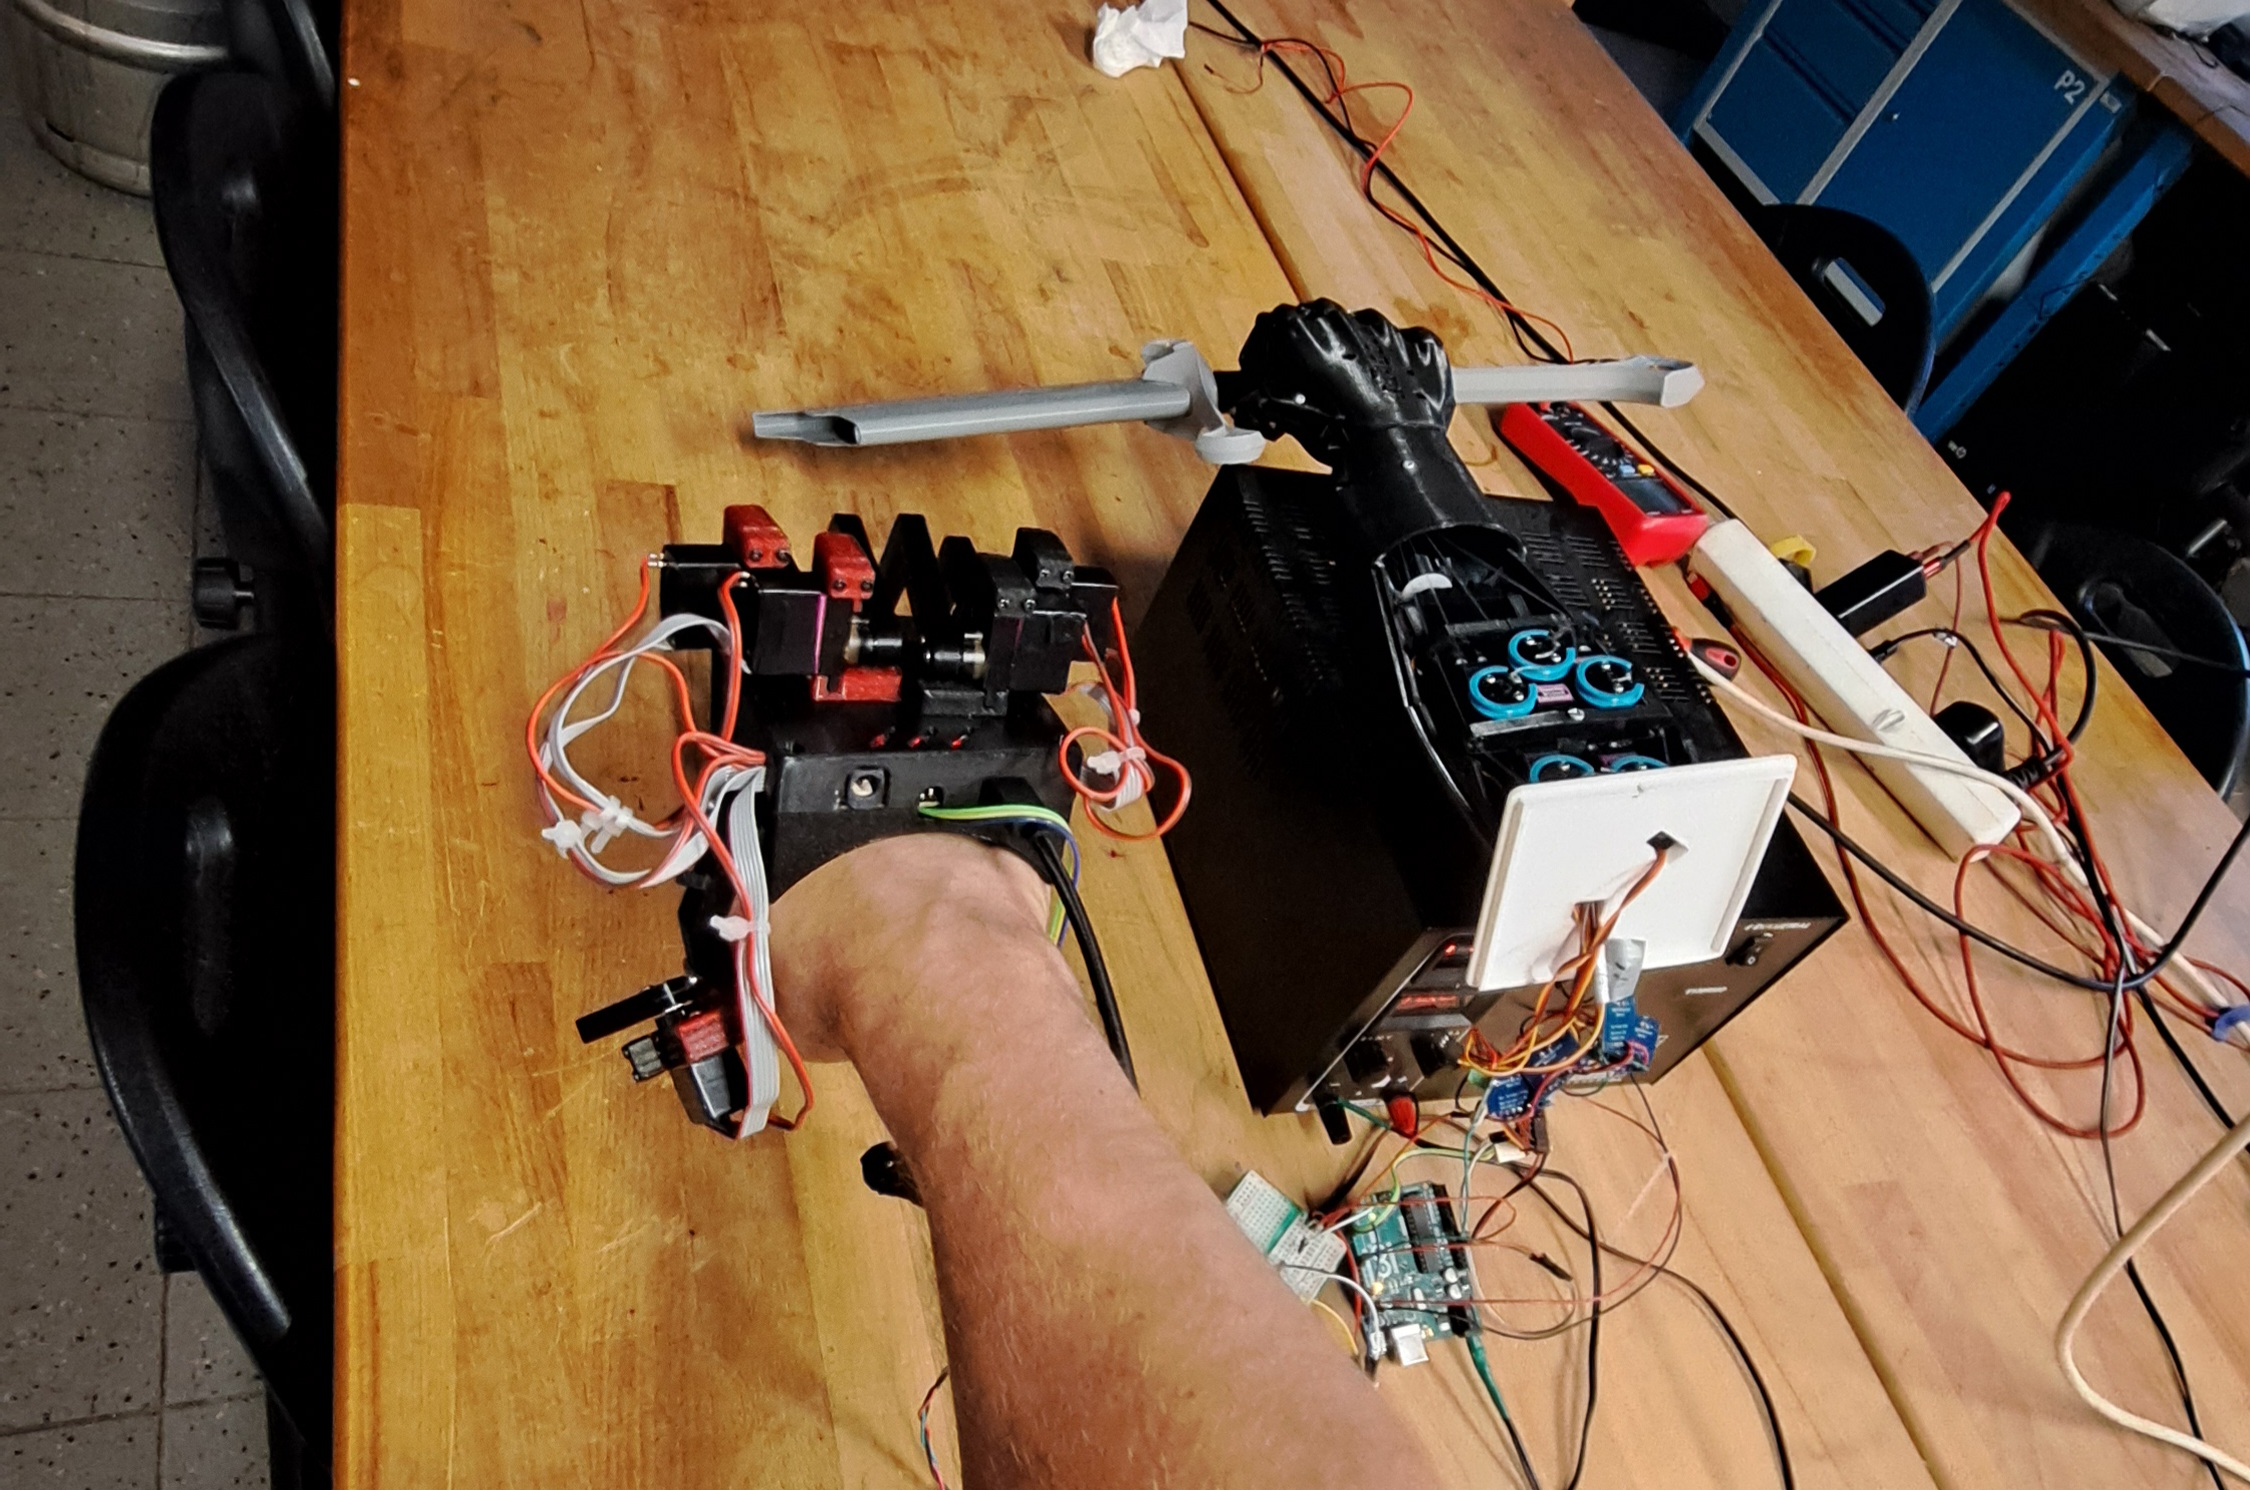
\includegraphics[width=0.9\textwidth]{drzi_mec.jpg}
\caption{Testování držení plastového meče.}
\end{figure}

V režimu EMG bylo praktické uchopení předmětů výrazně méně spolehlivé než v režimu MIRROR\@. Houbičku na nádobí se podařilo úspěšně uchopit pouze v jednom ze tří pokusů, plastový meč ve dvou ze tří pokusů a fixu se nepodařilo uchopit vůbec. Subjektivní praktičnost režimu EMG byla hodnocena 2/5.

Režim EMG byl při uchopování použitelný pouze omezeně, zejména kvůli nestabilnímu úchopu, nechtěným pohybům a obtížnému udržení jiné než krajní polohy.

\section{Pozorování rušení EMG signálu}
\label{sec:ruseni-emg}

Měření M9 bylo zaměřeno na pozorování rušení EMG signálu. V klidu bez pohybu kabelů docházelo k občasné aktivaci. Pohyb kabelů sEMG měl výrazný vliv na chování systému. Přiblížení k napájení nebo elektronice mělo menší vliv. Nejčastějším projevem rušení bylo cukání a samovolné zavření robotické ruky. Bluetooth spojení bylo během testu stabilní.

Bylo zaznamenáno, že senzor MyoWare neměl kabely připojené napevno. Při pohybu se proto kabely mohly pohybovat a způsobovat rušení nebo úplné přerušení signálu. Subjektivní odolnost EMG proti rušení byla hodnocena 1/5.

Pozorované problémy byly přisouzeny primárně sEMG signálu a kabeláži, nikoli komunikaci mezi deskami. Tato interpretace byla podpořena tím, že Bluetooth spojení zůstalo během měření stabilní.

\section{Subjektivní hodnocení režimů řízení}
\label{sec:subjektivni-hodnoceni}

Po dokončení dílčích měření bylo provedeno subjektivní hodnocení obou režimů. Hodnocena byla přirozenost ovládání, přesnost, rychlost, únava, pocit kontroly, praktičnost pro uchopení předmětů a celkové hodnocení. U kritéria únavy znamenala hodnota 1 velkou únavu a hodnota 5 stav bez únavy.

\begin{table}[htbp]
\centering
\caption{Subjektivní hodnocení režimů MIRROR a EMG}
\label{tab:subjektivni-hodnoceni}
\begin{tabular}{|p{0.55\textwidth}|p{0.17\textwidth}|p{0.17\textwidth}|}
\hline
\textbf{Kritérium} & \textbf{MIRROR} & \textbf{EMG} \\
\hline
Přirozenost ovládání & 4/5 & 2/5 \\
\hline
Přesnost & 5/5 & 1/5 \\
\hline
Rychlost & 4/5 & 4/5 \\
\hline
Únava & 3/5 & 2/5 \\
\hline
Pocit kontroly & 3/5 & 2/5 \\
\hline
Praktičnost pro uchopení předmětů & 5/5 & 2/5 \\
\hline
Celkové hodnocení & 4/5 & 2/5 \\
\hline
\end{tabular}
\end{table}

Režim MIRROR byl slovně hodnocen jako dobrý základ pro teleoperativní úlohy. Režim EMG byl hodnocen jako funkční, ale pro spolehlivé řízení vyžadující další odladění více částí systému. Subjektivní hodnocení potvrdilo objektivní pozorování z dílčích testů: MIRROR byl hodnocen lépe v přesnosti, přirozenosti i praktičnosti uchopení.

\section{Diskuse výsledků}
\label{sec:diskuse-vysledku}

Testováním bylo ukázáno, že režim MIRROR poskytoval výrazně spolehlivější, přesnější a lépe opakovatelné řízení robotické ruky než režim EMG\@. V dynamickém testu otevřít--zavřít--otevřít měl MIRROR průměrnou reakci přibližně 135~ms při zavření a 126~ms při otevření. Pohyb byl plynulý, dobře opakovatelný a Bluetooth spojení bylo stabilní.

Režim EMG měl ve stejném testu průměrnou reakci přibližně 546~ms při zavření a 553~ms při otevření. Prakticky byl však výrazně omezen nestabilitou sEMG signálu, pohybovými artefakty kabeláže a samovolnými aktivacemi. Jemné řízení mezilehlé polohy bylo u EMG nespolehlivé.

Při uchopování předmětů byl režim MIRROR použitelnější a praktičtější. Umožnil přirozenější dávkování sevření a lepší kontrolu nad okamžikem uchopení i puštění předmětu. Režim EMG byl použitelný pouze omezeně, zejména kvůli nestabilnímu úchopu a obtížnému udržení jiné než krajní polohy.

Bluetooth spojení bylo během měření stabilní. Pozorované problémy EMG řízení proto nebyly přisuzovány komunikaci mezi deskami, ale především kvalitě sEMG vstupu, mechanickému namáhání kabelů a citlivosti senzoru MyoWare 1.0 na pohybové artefakty.

\section{Souběžné využití MIRROR a EMG}
\label{sec:soubezne-vyuziti}

Souběžná činnost režimů MIRROR a EMG byla vyhodnocena jako potenciálně přínosná. Z hlediska řešené problematiky může sEMG poskytovat doplňující informaci využitelnou ke zlepšení silové zpětné vazby, odhadu únavy uživatele nebo řízení aktivní asistence rukavice.

Pro samotné řízení robotické ruky však testováním nebyl prokázán jasný důvod, proč by v aktuální podobě mělo sEMG nahrazovat řízení pomocí rukavice. Souběžná činnost MIRROR a EMG proto byla vyhodnocena jako perspektivní spíše pro doplňkovou analýzu než jako přímá náhrada polohového řízení.

\section{Dílčí závěr experimentální kapitoly}
\label{sec:dilci-zaver-experimenty}

Experimentálním testováním bylo prokázáno, že v aktuální podobě systému je režim MIRROR vhodnější pro řízení robotické ruky než režim EMG\@. Režim MIRROR vykazoval kratší reakční dobu, lepší opakovatelnost, vyšší stabilitu v klidu, lepší jemnou ovladatelnost a vyšší praktickou úspěšnost při uchopování předmětů.

Režim EMG byl funkční, avšak jeho praktické použití bylo výrazně omezeno nestabilitou sEMG signálu, pohybovými artefakty kabeláže a samovolnými aktivacemi. Souběžné využití EMG a MIRROR může být perspektivní zejména jako doplněk pro vyhodnocení únavy, podporu aktivní asistence rukavice nebo budoucí rozšíření silové zpětné vazby. V aktuální podobě však nebylo vhodné chápat EMG jako přímou náhradu řízení podle polohy prstů v rukavici.
